%%%%%%%%%%%%%%%%%%%%%%%%%%%%%%%%%%%%%%%%%%%%%%%%%%%%%%%%%%%%%%%%%%%%%%
% Problem statement
\begin{statement}[
  problempoints=100,
  timelimit=4 seconds,
  memorylimit=512 MiB,
]{Semafor}

You are most likely familiar with a so-called \textit{7-segment} display which
is widely used to depict digits on various digital devices, such as watches or
calculators. Due to its simplicity, intuitiveness and aestheticism, this design
has been accepted across the globe. Still, young Matej argues against the
7-segment design and claims that the same functionality can be obtained
more efficiently, using only 5 segments.

\begin{figure}[H]
  \begin{center}
    
\includegraphics[width=0.8\textwidth]{img/5segment.png}

    \vspace{0.5cm}

    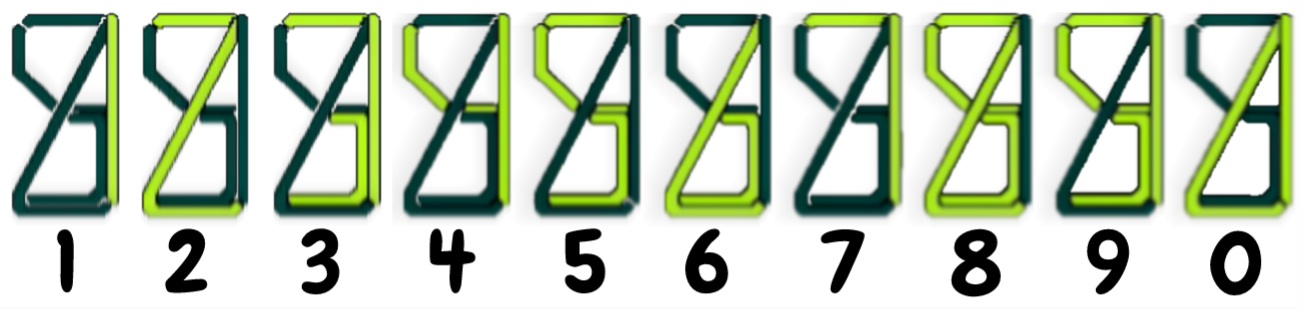
\includegraphics[width=0.8\textwidth]{img/5segmentdigits.png}
    \caption*{\textit{5-segment} display design -- segments are labeled using
              with letters from \texttt{a} to \texttt{e}.}
  \end{center}
\end{figure}
  \vspace{-0.7cm}
Matej decided to make his first entrepreneurial steps in the most prosperous
branch of Croatian economy, football. His revolutionary design will be used
on a substitution board during the games of 1.\ HNL.\footnote{The elite tier
of Croatian professional football.} He is currently making a presentation for
the board of directors at the Croatian Football Association.

The substitution board consists of $M$ 5-segment displays which, from left to
right, represent the digits of a jersey number worn by the player that is about
to leave the pitch. At the beginning of Matej's presentation, the substitution
board represents the number $X$, and Matej will make one of the following moves
each second:

\begin{itemize}
    \item Turn on one segment that is currently turned off.
    \item Turn off one segment that is currently turned on.
\end{itemize}

Also, Matej will make sure that after each $K$-th move, the board shows a valid
number. The number is valid if each of its digits is correctly shown on the
corresponding display (i.e. segments that are turned on show a valid digit).
Also, numbers having less than $M$ digits are validly shown if they contain
the appropriate number of leading zeros.

For each final state (integer between $0$ and $10^M-1$), Matej is interested
in how many different ways could he make his moves during the presentation such
that this final state is reached at the end. Of course, he needs to adhere to
all limitations presented in the previous chapters. We consider two sequences
of moves different if, imagining they are executed on two different boards
at the same time, there is a moment at which the two boards represent a different
state.

Since the number of different ways can be quite large, you are asked to compute
it modulo $10^9+7$.
\clearpage

%%%%%%%%%%%%%%%%%%%%%%%%%%%%%%%%%%%%%%%%%%%%%%%%%%%%%%%%%%%%%%%%%%%%%%
% Input
\subsection*{Input}
The first line contains integers $M$, $N$, $K$ $(1 \le K \le N)$ and $X$ $(0
\le X < 10^M)$ from the task description.

%%%%%%%%%%%%%%%%%%%%%%%%%%%%%%%%%%%%%%%%%%%%%%%%%%%%%%%%%%%%%%%%%%%%%%
% Output
\subsection*{Output}
In the $i$-th line you should output the number of different ways for the
substitution board to show the number $i-1$ at the end of Matej's presentations.
The numbers should be printed modulo $10^9 + 7$.

%%%%%%%%%%%%%%%%%%%%%%%%%%%%%%%%%%%%%%%%%%%%%%%%%%%%%%%%%%%%%%%%%%%%%%
% Scoring
\subsection*{Scoring}
{\renewcommand{\arraystretch}{1.4}
  \setlength{\tabcolsep}{6pt}
  \begin{tabular}{ccl}
 Subtask & Score & Constraints \\ \midrule
  1 & 6 & $M=1$, $1 \le N \le 12$ \\
  2 & 15 & $M=1$, $1 \le N \le 10^{15}$ \\
  3 & 12 & $M=2$, $1 \le N \le 1\,500$, $K = N$\\
  4 & 12 & $M=2$, $1 \le N \le 10^{15}$, $1 \le K \le 15$ \\
  5 & 15 & $M=2$, $1 \le N \le 10^{15}$, $1 \le K \le 1\,500$ \\
  6 & 40 & $M=2$, $1 \le N \le 10^{15}$ \\
\end{tabular}}

%%%%%%%%%%%%%%%%%%%%%%%%%%%%%%%%%%%%%%%%%%%%%%%%%%%%%%%%%%%%%%%%%%%%%%
% Examples
\subsection*{Examples}
\begin{tabularx}{\textwidth}{X'X'X}
\sampleinputs{test/semafor.dummy.in.1}{test/semafor.dummy.out.1} &
\sampleinputs{test/semafor.dummy.in.2}{test/semafor.dummy.out.2} &
\sampleinputs{test/semafor.dummy.in.3}{test/semafor.dummy.out.3}
\end{tabularx}

\textbf{Clarification of the first example:}
At the beginning of the presentation the (single-digit) substitution board
shows the number $5$. After each move (due to $K=1$), the board must show
a valid number. Matej is going to make a total of $N=2$ moves. Therefore,
at the end of the presentation, the board can show either number $3$ or
number $5$. Number $3$ can be obtained using one way ($5-9-3$) and number $5$
can be obtained using two ways ($5-9-5$ and $5-8-5$).

%%%%%%%%%%%%%%%%%%%%%%%%%%%%%%%%%%%%%%%%%%%%%%%%%%%%%%%%%%%%%%%%%%%%%%
% We're done
\end{statement}

%%% Local Variables:
%%% mode: latex
%%% mode: flyspell
%%% ispell-local-dictionary: "croatian"
%%% TeX-master: "../hio.tex"
%%% End:
